% ★★ 中档
\newcommand{\qConicDefThreeEllipseSymmetryStem}{
已知 $A, B$ 是椭圆 $\frac{x^2}{a^2} + \frac{y^2}{b^2} = 1\ (a > b > 0)$ 上关于原点对称的两个点，$P$ 是椭圆上异于 $A, B$ 的任意一点．若 $PA$ 和 $PB$ 的斜率存在，求证：斜率乘积 $k_{PA} \cdot k_{PB}$ 为定值 $-\frac{b^2}{a^2}$．
}
\newcommand{\qConicDefThreeEllipseSymmetryFigure}{
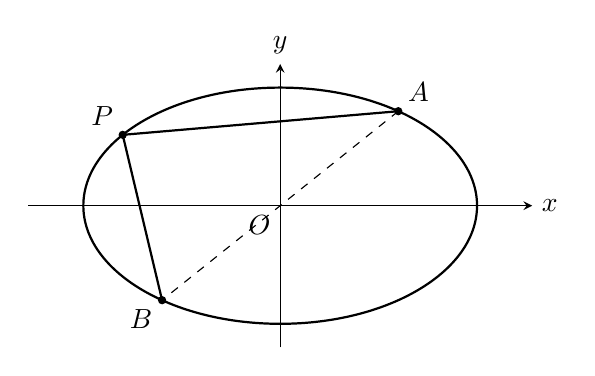
\begin{tikzpicture}[scale=1, >=stealth]
  % Axes
  \draw[->] (-3.2,0) -- (3.2,0) node[right] {$x$};
  \draw[->] (0,-1.8) -- (0,1.8) node[above] {$y$};
  \node[below left] at (0,0) {$O$};
  
  % Ellipse
  \draw[thick] (0,0) ellipse (2.5 and 1.5);
  
  % Symmetric points A, B
  \coordinate (A) at (1.5, 1.2);
  \coordinate (B) at (-1.5, -1.2);
  \fill (A) circle (1.5pt) node[above right] {$A$};
  \fill (B) circle (1.5pt) node[below left] {$B$};
  \draw[dashed] (A) -- (B);
  
  % Point P
  \coordinate (P) at (-2, 0.9);
  \fill (P) circle (1.5pt) node[above left] {$P$};
  
  % Lines
  \draw[thick] (P) -- (A);
  \draw[thick] (P) -- (B);
\end{tikzpicture}
}
\newcommand{\qConicDefThreeEllipseSymmetryAnswer}{
证明见解析．斜率积为定值 $-\frac{b^2}{a^2}$．
}
\newcommand{\qConicDefThreeEllipseSymmetrySolution}{
\begin{proof*}
设点 $A(x_1, y_1)$，因为点 $B$ 与点 $A$ 关于原点对称，则点 $B$ 的坐标为 $B(-x_1, -y_1)$．\\
设动点 $P(x_0, y_0)$．由题意，$PA$ 和 $PB$ 的斜率存在，故 $x_0 \neq \pm x_1$．\\
根据斜率公式：
\[
k_{PA} = \frac{y_0 - y_1}{x_0 - x_1}
\]
\[
k_{PB} = \frac{y_0 - (-y_1)}{x_0 - (-x_1)} = \frac{y_0 + y_1}{x_0 + x_1}
\]
两斜率的乘积为：
\[
k_{PA} \cdot k_{PB} = \frac{y_0 - y_1}{x_0 - x_1} \cdot \frac{y_0 + y_1}{x_0 + x_1} = \frac{y_0^2 - y_1^2}{x_0^2 - x_1^2}
\]
由于点 $P(x_0, y_0)$ 和点 $A(x_1, y_1)$ 均在椭圆 $\frac{x^2}{a^2} + \frac{y^2}{b^2} = 1$ 上，所以满足：
\[
\frac{x_0^2}{a^2} + \frac{y_0^2}{b^2} = 1 \implies \frac{y_0^2}{b^2} = 1 - \frac{x_0^2}{a^2} \quad \text{---(1)}
\]
\[
\frac{x_1^2}{a^2} + \frac{y_1^2}{b^2} = 1 \implies \frac{y_1^2}{b^2} = 1 - \frac{x_1^2}{a^2} \quad \text{---(2)}
\]
(1)式减去(2)式得：
\[
\frac{y_0^2 - y_1^2}{b^2} = -\frac{x_0^2 - x_1^2}{a^2}
\]
整理变形得：
\[
\frac{y_0^2 - y_1^2}{x_0^2 - x_1^2} = -\frac{b^2}{a^2}
\]
将上式代入斜率积公式中即可得：
\[
k_{PA} \cdot k_{PB} = -\frac{b^2}{a^2}
\]
因为 $a, b$ 为常数，所以斜率乘积 $k_{PA} \cdot k_{PB}$ 为定值 $-\frac{b^2}{a^2}$．
\end{proof*}
}
\newcommand{\qConicDefThreeEllipseSymmetryDiagnosis}{
\errortag{点差法两式相减失误} 此证明本质就是经典的“点差法”．学生在进行 (1)(2) 两式相减时，极易将符号弄错，导致得出 $\frac{b^2}{a^2}$（漏掉了负号）．\\
\errortag{对称点设定混乱} 少数学生可能会将 $B$ 的坐标错误地设为 $(x_1, -y_1)$（关于 $x$ 轴对称）或 $(-x_1, y_1)$（关于 $y$ 轴对称），没有理解“关于原点对称”的代数表示为 $(-x_1, -y_1)$．
}
